\documentclass[12pt, a4paper]{article}
\usepackage[utf8]{inputenc}
\usepackage{geometry}
\geometry{a4paper, margin=1in}
\usepackage{hyperref}
\usepackage{titlesec}
\usepackage{parskip}
\usepackage{tikz}
\usetikzlibrary{shapes.geometric, arrows.meta, positioning, fit, backgrounds}

\title{\textbf{DNA Data Storage Codec System}\\ \Large Project Progress \& Architecture Report}
\author{}
\date{\today}

\begin{document}

\maketitle

\section*{1. The Vision and Objective}
We are building a comprehensive \textbf{DNA Data Storage Codec System}. As global data generation accelerates, traditional silicon and magnetic storage media are failing to keep pace in terms of density and longevity. DNA represents the ultimate storage medium—capable of storing millions of terabytes in a single drop of liquid with a half-life of thousands of years. 

The objective of this project is to build a world-class, end-to-end software pipeline capable of translating arbitrary digital files (e.g., images, text documents) into biological DNA sequences, and leveraging Artificial Intelligence to reliably recover that data despite natural biological mutations.

\section*{2. The Core Biological Challenge}
Converting binary data ($0$s and $1$s) directly into nucleotide bases (A, C, G, T) is biologically unviable. Unconstrained mapping leads to unstable DNA sequences, particularly \textit{homopolymers} (e.g., AAAAA), which cause physical synthesis and sequencing equipment to crash. Furthermore, sequences must maintain a Guanine-Cytosine (GC) content of approximately 50\% to prevent the DNA from physically melting or forming secondary structures. Finally, the physical reading process (sequencing) introduction of massive noise in the form of insertion, deletion, and substitution mutations.

\section*{3. System Architecture Diagram}

\begin{figure}[h]
\centering
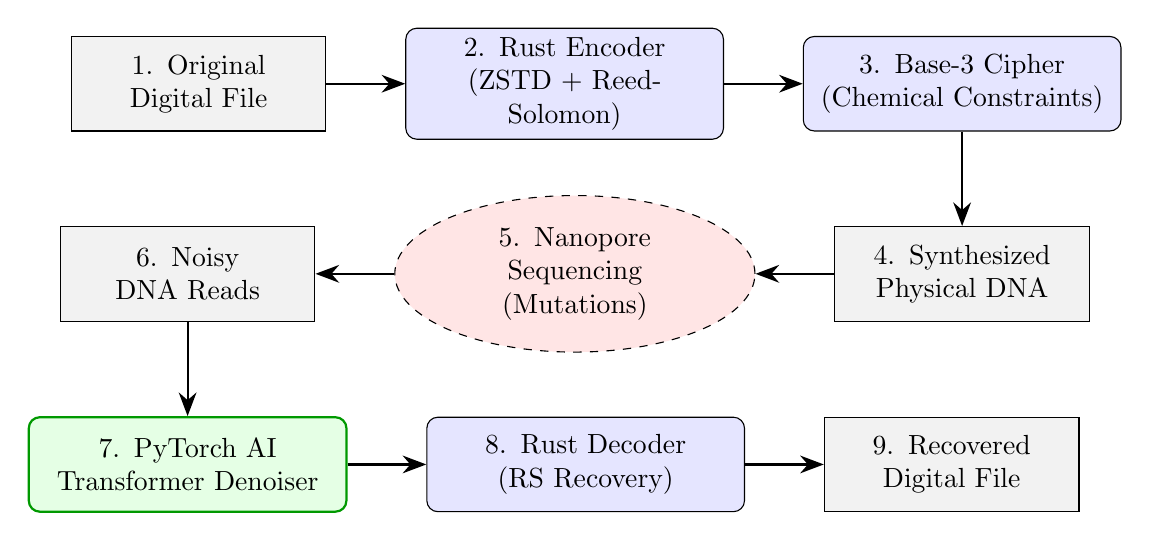
\begin{tikzpicture}[
    node distance=1.2cm and 1cm,
    box/.style={rectangle, draw, rounded corners, fill=blue!10, text width=3.8cm, align=center, minimum height=1.2cm},
    ai_box/.style={rectangle, draw, rounded corners, fill=green!10, text width=3.8cm, align=center, minimum height=1.2cm, thick, draw=green!60!black},
    noise_box/.style={ellipse, draw, fill=red!10, text width=3cm, align=center, minimum height=1.2cm, dashed},
    data/.style={rectangle, draw, fill=gray!10, text width=3cm, align=center, minimum height=1.2cm},
    arrow/.style={-{Stealth[length=3mm]}, thick}
]

% Top Row (Encoding)
\node[data] (input) {1. Original Digital File};
\node[box, right=of input] (rust_enc) {2. Rust Encoder\\(ZSTD + Reed-Solomon)};
\node[box, right=of rust_enc] (cipher) {3. Base-3 Cipher\\(Chemical Constraints)};

% Middle Row (Physical/Biological)
\node[data, below=of cipher] (dna) {4. Synthesized Physical DNA};
\node[noise_box, left=of dna] (sequencer) {5. Nanopore Sequencing\\(Mutations)};
\node[data, left=of sequencer] (noisy) {6. Noisy DNA Reads};

% Bottom Row (Decoding)
\node[ai_box, below=of noisy] (ai) {7. PyTorch AI\\Transformer Denoiser};
\node[box, right=of ai] (rust_dec) {8. Rust Decoder\\(RS Recovery)};
\node[data, right=of rust_dec] (output) {9. Recovered Digital File};

% Connections
\draw[arrow] (input) -- (rust_enc);
\draw[arrow] (rust_enc) -- (cipher);
\draw[arrow] (cipher) -- (dna);
\draw[arrow] (dna) -- (sequencer);
\draw[arrow] (sequencer) -- (noisy);
\draw[arrow] (noisy) -- (ai);
\draw[arrow] (ai) -- (rust_dec);
\draw[arrow] (rust_dec) -- (output);

\end{tikzpicture}
\caption{End-to-End DNA Data Storage Pipeline}
\end{figure}

\section*{4. Current Progress: Completed Milestones}
We have successfully completed Phase 1: \textbf{The Encoding and Visualization Pipeline}.

\begin{itemize}
    \item \textbf{The Core Engine (Rust):} We engineered an ultra-fast, highly optimized backend codec using the Rust programming language. The engine compresses input files using ZSTD and wraps the payload in heavy mathematical error correction (Reed-Solomon) to protect against degradation.
    
    \item \textbf{Biological Constraints Engine:} We designed and implemented a custom \textit{Base-3 Rotating Cipher}. This mathematical layer guarantees that the output DNA is chemically stable by strictly preventing homopolymers and enforcing ideal GC content ratios.
    
    \item \textbf{Professional Graphical Interface (PyQt6):} We built a hardware-accelerated Native Desktop Application. It provides a highly interactive interface where users can upload files and visually inspect the generated DNA. The software renders the DNA as an interactive 3D matrix, complete with real-time chemical analysis (molar mass, hydrogen bonding, and structural class) of individual nucleotide molecules.
    
    \item \textbf{Synthesis Export:} The software includes an export module that formats the generated DNA into industry-standard \texttt{.FASTA} files, ready for commercial biological synthesis (e.g., Twist Bioscience).
    
    \item \textbf{AI Training Data Generation:} To prepare for Phase 2, we built a biological noise simulator that mimics real-world nanopore sequencer errors, successfully generating a dataset of over 100,000 synthetic mutated DNA strands.
\end{itemize}

\section*{5. Next Steps: The AI Recovery Pipeline}
With the Encoder complete, our next focus is Phase 2: \textbf{The Decoder and AI Denoiser}.

Due to the massive alignment errors introduced by physical DNA sequencers, traditional mathematical decoders struggle to recover the data alone. To solve this, we are building a \textbf{Deep Learning Transformer Model} using PyTorch (utilizing a Sequence-to-Sequence architecture). 

This neural network will act as an intelligent biological error-correction system. It will ingest the noisy, mutated DNA reads from the laboratory, mathematically align and fix the biological errors, and output pristine DNA sequences. These cleaned sequences will then be passed back to our Rust engine to perfectly extract and reconstruct the original digital file.

\end{document}
